\documentclass{article}
\usepackage[a4paper, total={6in, 9in}]{geometry}
\usepackage{fancyhdr}
\usepackage{amsmath}
\usepackage{algorithm}
\usepackage{algpseudocode}
\usepackage{CJK}
\usepackage{graphicx}

\newtheorem{theorem}{Theorem}
\newtheorem{lemma}{Lemma}
\newtheorem{proof}{Proof}[section]

\pagestyle{fancy}
\fancyhf{}
\rhead{1600017857}
\lhead{Homework(2)}
\rfoot{}
\cfoot{Page \thepage}

\title{Homework(2)}
\date{2018-03-02}
\author{
  \begin{CJK}{UTF8}{gbsn}
    黄道吉-1600017857
  \end{CJK}
}

\begin{document}
\section{Q1}
  \paragraph{$\mathcal{C}_1 = \phi$}
    is open, close, bounded and compact, its interior, closure, boundary and accumulation point set is $\phi$.
  \paragraph{$\mathcal{C}_2 = \mathcal{R}^n$}
    is open, close, not bounded and thus not compact, its interior, closure, boundary and accumulation points set is $\mathcal{R}^n$ .
  \paragraph{$\mathcal{C}_3 = [0, 1) \cup [2, 3] \cup (4, 5]$}
    is not open, not close, is bounded, but not compact, its interior is $(0, 1) \cup (2, 3) \cup (4, 5)$, its closure is $[0, 1] \cup [2, 3] \cup [4, 5]$, its boundary is $\{0, 1, 2, 3, 4, 5\}$, and its accumulation points are $[0, 1] \cup [2, 3] \cup [4, 5]$.
  \paragraph{$\mathcal{C}_4 = \{(x, y)^T |\  x \geq 0, y > 0\}$}
    is not open, not close, not bounded, not compact, and its interior is $\{(x, y)|\ x > 0, y > 0\}$, its closure is $\{(x, y)|\ x \ge 0, y \ge 0\}$, its boundary is $\{(0, y)|y \ge 0 \} \cup \{(x, 0)|\ x \ge 0\}$, and is accumulation points is $\{(x, y)|\ x \ge 0, y \ge 0\}$.
  \paragraph{$\mathcal{C}_5 = \{k|\ k \in \mathcal{Z}\}$}
    is not open, but is  closed, is not bounded, and not compact, its interior is $\phi$, its closure and boundary is itself, $\{k|\ k \in \mathcal{Z}\}$, and its accumulation points are $\phi$.
  \paragraph{$\mathcal{C}_6 = \{k^{-1}|\ k \in \mathcal{Z}\}$}
    is not open, not closed, but is bounded, and is not compact, its interior is $\phi$, its closure and boundary is $\{k^{-1}|\ k \in \mathcal{Z}\} \cup \{0\}$, its accumulation point is $\{0\}$.
  \paragraph{$\mathcal{C}_7 = \{(1 / k, \sin{k}^T|\ k \in \mathcal{Z})\}$}
    is not open, not closed, but is bounded, and is not compact, its interior is $\phi$, its closure and boundary are $\{(1 / k, \sin{k}^T|\ k \in \mathcal{Z})\} \cup \{(0, y)|\ -1 \leq y \leq 1\}$, and its accumulation points are $\{(0, y)|\ -1 \leq y \leq 1\}$.

\section{Q2}
  \paragraph{}
    1. suppose $\mathcal{C}$ is closed, if there exists $x^*$ which is the limit of one convergent sequence in $\mathcal{C}$, but $x^* \not\in \mathcal{C}$, thus $x^* \in \mathcal{C}^c$, which is an open set, so we have
    \begin{equation}
      \exists \epsilon\ s.t.\ (\cup(x^*, \epsilon)) \cap \mathcal{C} = \phi
    \end{equation}
    for we have $\cup(x^*, \epsilon) \subseteq \mathcal{C}^c$. but there exists $\{x_k\}_1^{\infty} \subseteq \mathcal{C}$ s.t. $\lim_{k \to \infty} x_k = x^*$, that is to say,
    \begin{equation}
      \forall \epsilon\ \ (\cup(x^*, \epsilon)) \cap \mathcal{C} \not= \phi
    \end{equation}
    contradiction! so for all $x^*$ which is the limit of one convergent sequence in $\mathcal{C}$, we have $x^* \in \mathcal{C}$
    \paragraph{}
      2. if $\mathcal{C}$ contains the limit point of every convergent sequence in it, suppose $\mathcal{C}$ is not closed, $i.e.$ $\mathcal{C}^c$ is not open, that is to say,
      \begin{equation}
        \exists x^* \in \mathcal{C}^c\ \forall\ \epsilon > 0\ (\cup(x^*, \epsilon)) \cap \mathcal{C} \not= \phi
      \end{equation}
      for we have $(\mathcal{C}^c)^c = \mathcal{C}$. so we choose a sequence of $\epsilon_k \to 0$ and find $x_k \in (\cup(x^*, \epsilon)) \cap \mathcal{C}$, then $lim_{k \to \infty} x_k = x^*$, so $x^* \in \mathcal{C}$, contradiction! so $\mathcal{C}$ must be closed.
    \paragraph{}
      3. from 1 and 2, we have a set $\mathcal{C} \subseteq \mathcal{R}^n$ is closed iff it contains the limit point of every convergent sequence in it.

\section{Q3}
  \paragraph{}
  $x$ $\in$ $\partial\mathcal{C} = \bar{\mathcal{C}} \setminus \mathcal{C}^o = ((\mathcal{C}^c)^o)^c \setminus \mathcal{C}^o = ((\mathcal{C}^c)^o)^c \cap (\mathcal{C}^o)^c$
  \paragraph{}
    by definition, $x \in \mathcal{C}^o \iff \exists \epsilon > 0\ \cup(x, \epsilon) \subseteq \mathcal{C}$, thus we have
    \begin{equation}
      x \in (\mathcal{C}^o)^c\ \iff\ \forall \epsilon > 0\ \exists z \not\in \mathcal{C}\ |z - x|_2 < \epsilon
    \end{equation}
    and if we change $\mathcal{C}^o$ in equation (4) into $(\mathcal{C}^c)^o$, we have
    \begin{equation}
      x \in ((\mathcal{C}^c)^o)^c\ \iff\ \forall \epsilon > 0\ \exists y \in \mathcal{C}\ |y - x|_2 < \epsilon
    \end{equation}
  \paragraph{}
    so $x$ $\in$ $\partial\mathcal{C} = ((\mathcal{C}^c)^o)^c \cap (\mathcal{C}^o)^c \iff \forall \epsilon > 0\ \exists y \in \mathcal{C}\ |y - x|_2 < \epsilon\ \exists z \not\in \mathcal{C}\ |z - x|_2 < \epsilon$

\section{Q4}
  \paragraph{1.1} if $\mathcal{C}$ is closed,  then for all $x^*$ in $\partial \mathcal{C}$, from $Q3$, we have $\forall \epsilon > 0\ \exists y \in \mathcal{C}\ |y - x^*|_2 < \epsilon$, then $x^*$ must be a limit of one convergent sequence in $\mathcal{C}$, then from $Q2$, we have $x^* \in \mathcal{C}$, so $\mathcal{C} \supseteq \partial \mathcal{C}$.
  \paragraph{1.2} if $\mathcal{C} \supseteq \partial \mathcal{C}$, suppose $\mathcal{C}$ is not closed, from $Q2$, there exists one point $x^*$ which is a limit of one convergent sequence in $\mathcal{C}$, but $x^* \not\in \mathcal{C}$, then we have
  \begin{equation}
    \forall \epsilon > 0\ \exists y \in \mathcal{C}\ |y - x^*|_2 < \epsilon\ \exists z \not\in \mathcal{C}\ |z - x^*|_2 < \epsilon,
  \end{equation}
  we can just choose $z = x^*$, then from $Q3$, $x^* \in \partial \mathcal{C} \subseteq \mathcal{C}$, contradiction! so $\mathcal{C}$ nust be closed.
  \paragraph{2.1} if $\mathcal{C}$ is open, suppose there exists $x^* \in \mathcal{C} \cap \partial \mathcal{C}$, then $\exists \epsilon > 0\ \cup(x^*, \epsilon) \subseteq \mathcal{C}$ and $\forall \epsilon > 0\ \exists z \not\in \mathcal{C}\ |z - x^*|_2 < \epsilon$, contradiction! so $\mathcal{C} \cap \partial \mathcal{C} = \phi$.
  \paragraph{2.2} if $\mathcal{C} \cap \partial \mathcal{C} = \phi$, suppose $\mathcal{C}$ is not open, $i.e.$ $\exists x^* \in \mathcal{C}\  \forall \epsilon > 0\ \exists z \not\in \mathcal{C}\ |z - x^*|_2 < \epsilon$, then from $Q3$, $x^* \in \partial \mathcal{C}$
  , contradiction! so $\mathcal{C}$ is open.
\begin{CJK}{UTF8}{gbsn}
\section{Q5, 6, 7的答案(图片)}
\end{CJK}
\begin{figure}[ht]
  \centering
  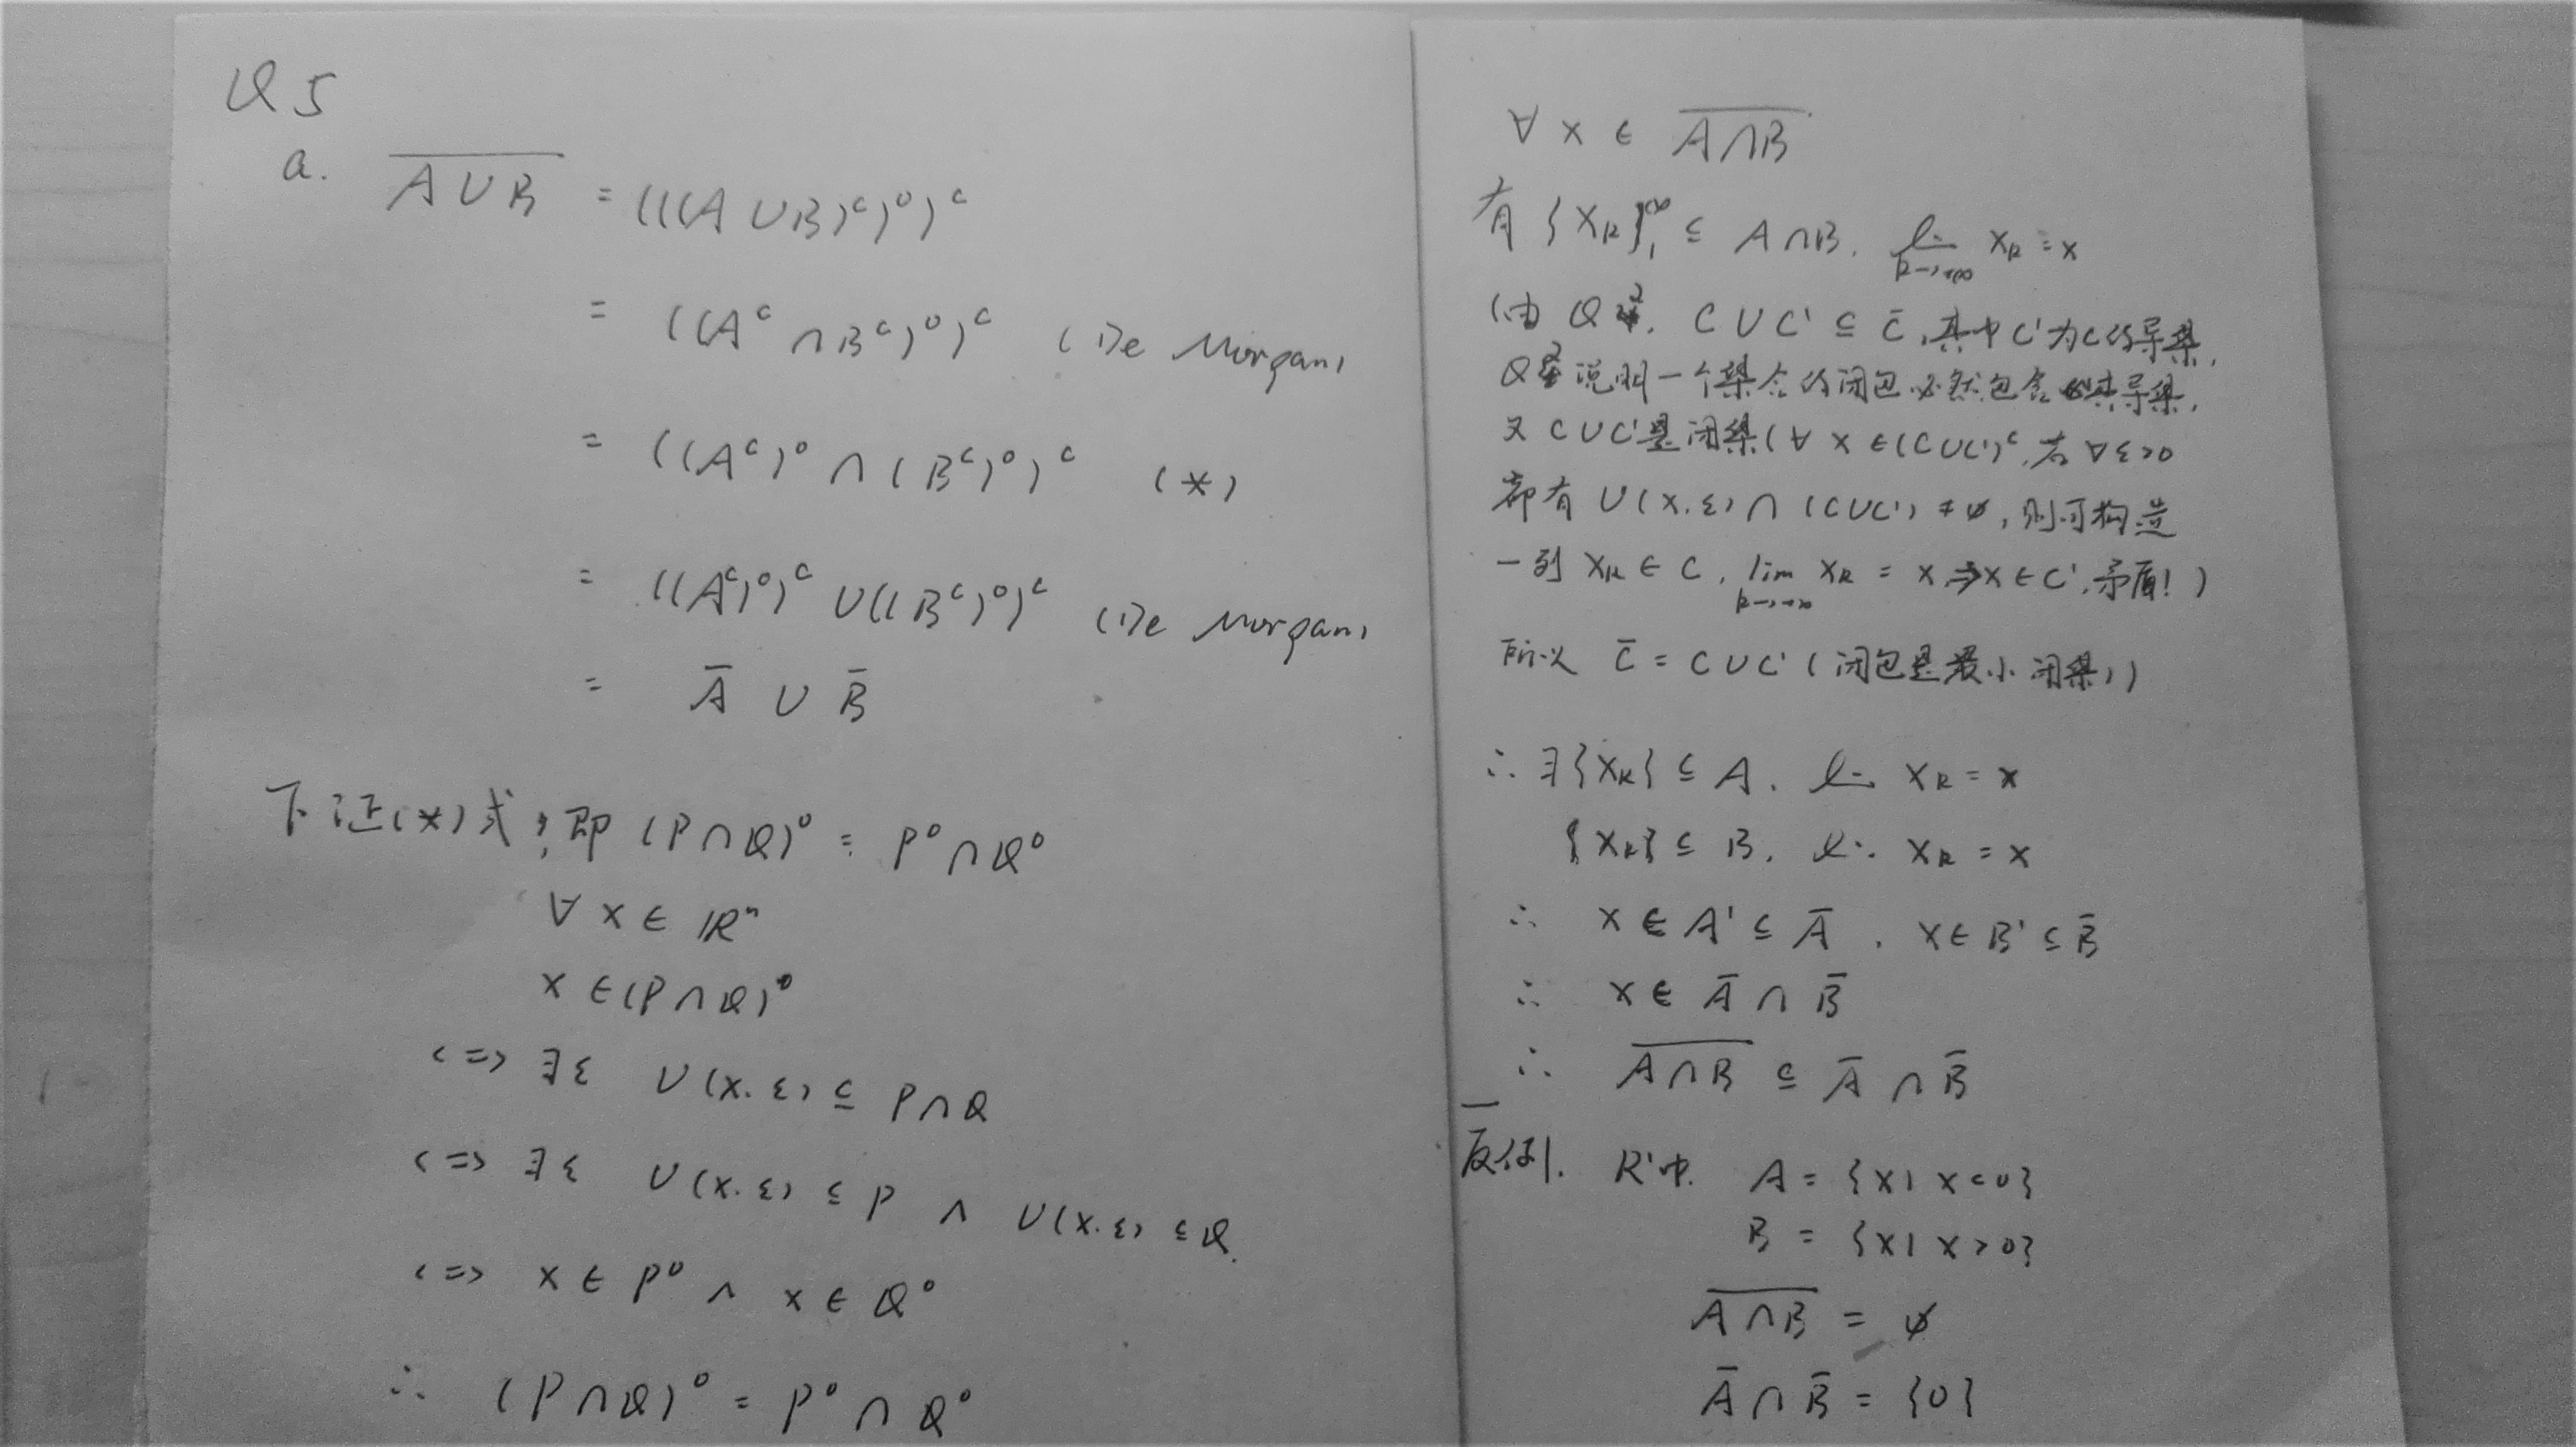
\includegraphics[scale=0.1]{Q5.jpg}
  \caption{Q5a}
  \label{fig:label}
\end{figure}

\begin{figure}[ht]
  \centering
  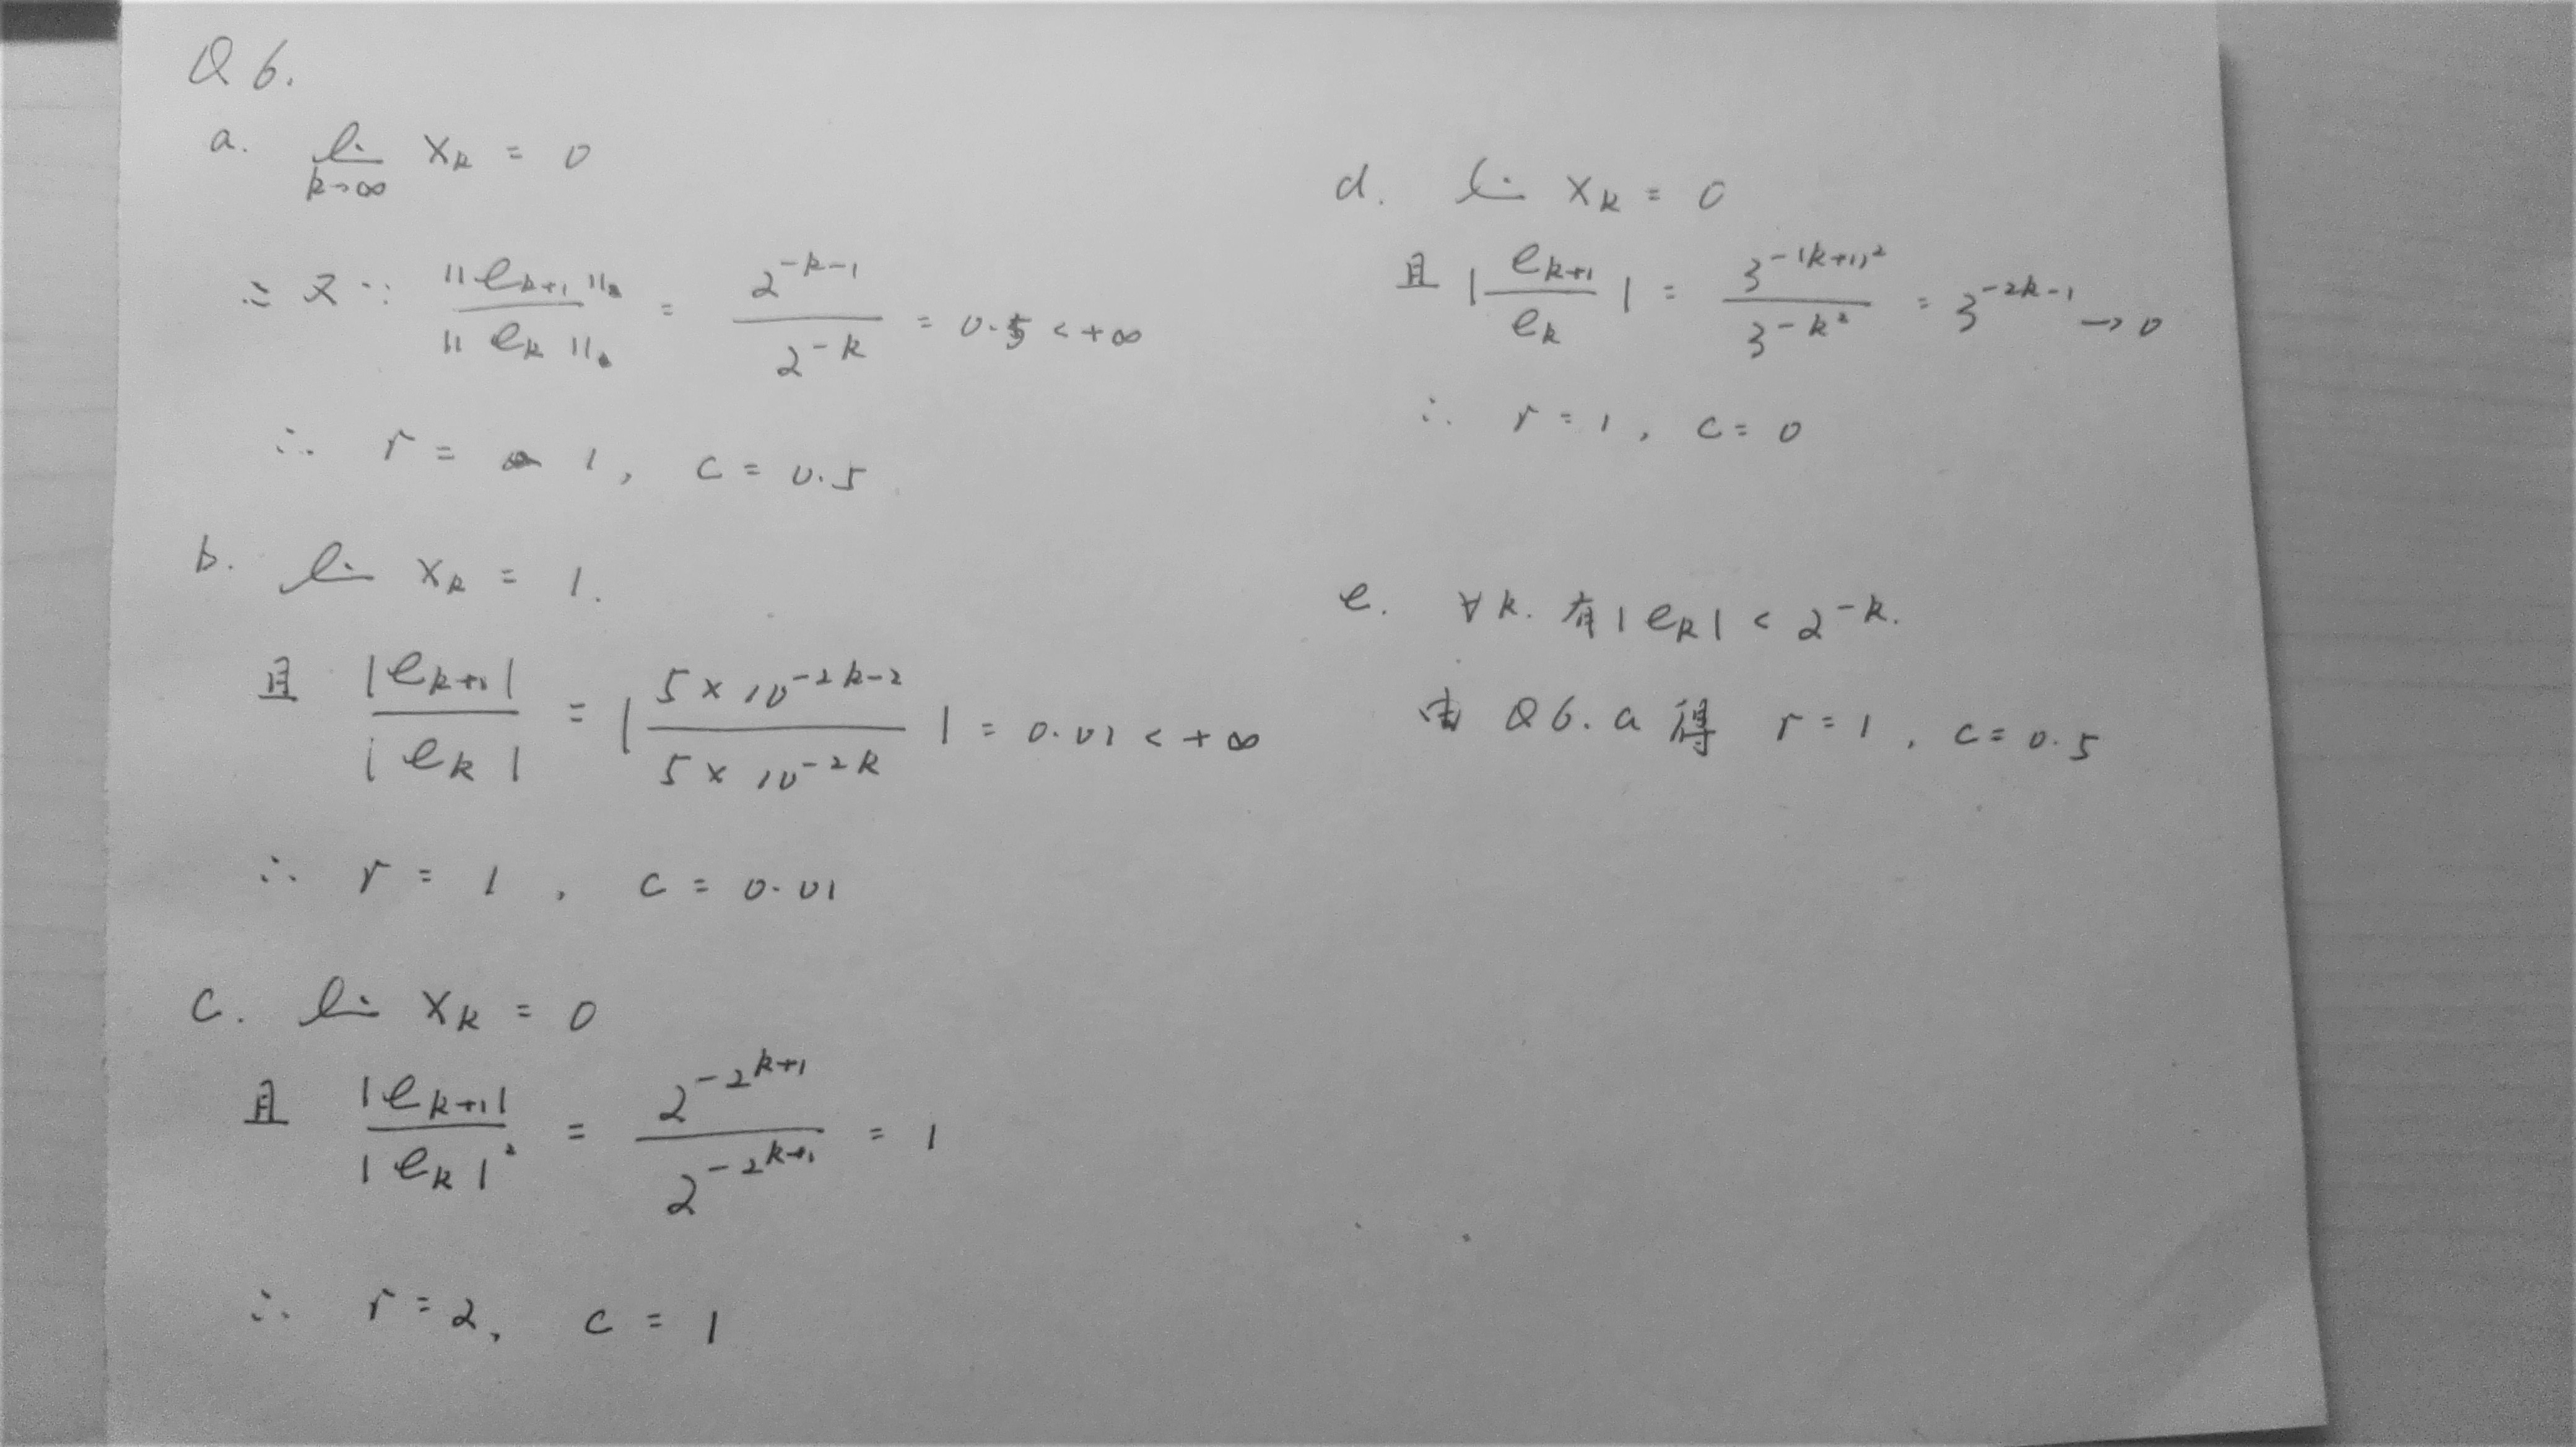
\includegraphics[scale=0.1]{Q6.jpg}
  \caption{Q6}
  \label{fig:label}
\end{figure}

\begin{figure}[ht]
  \centering
  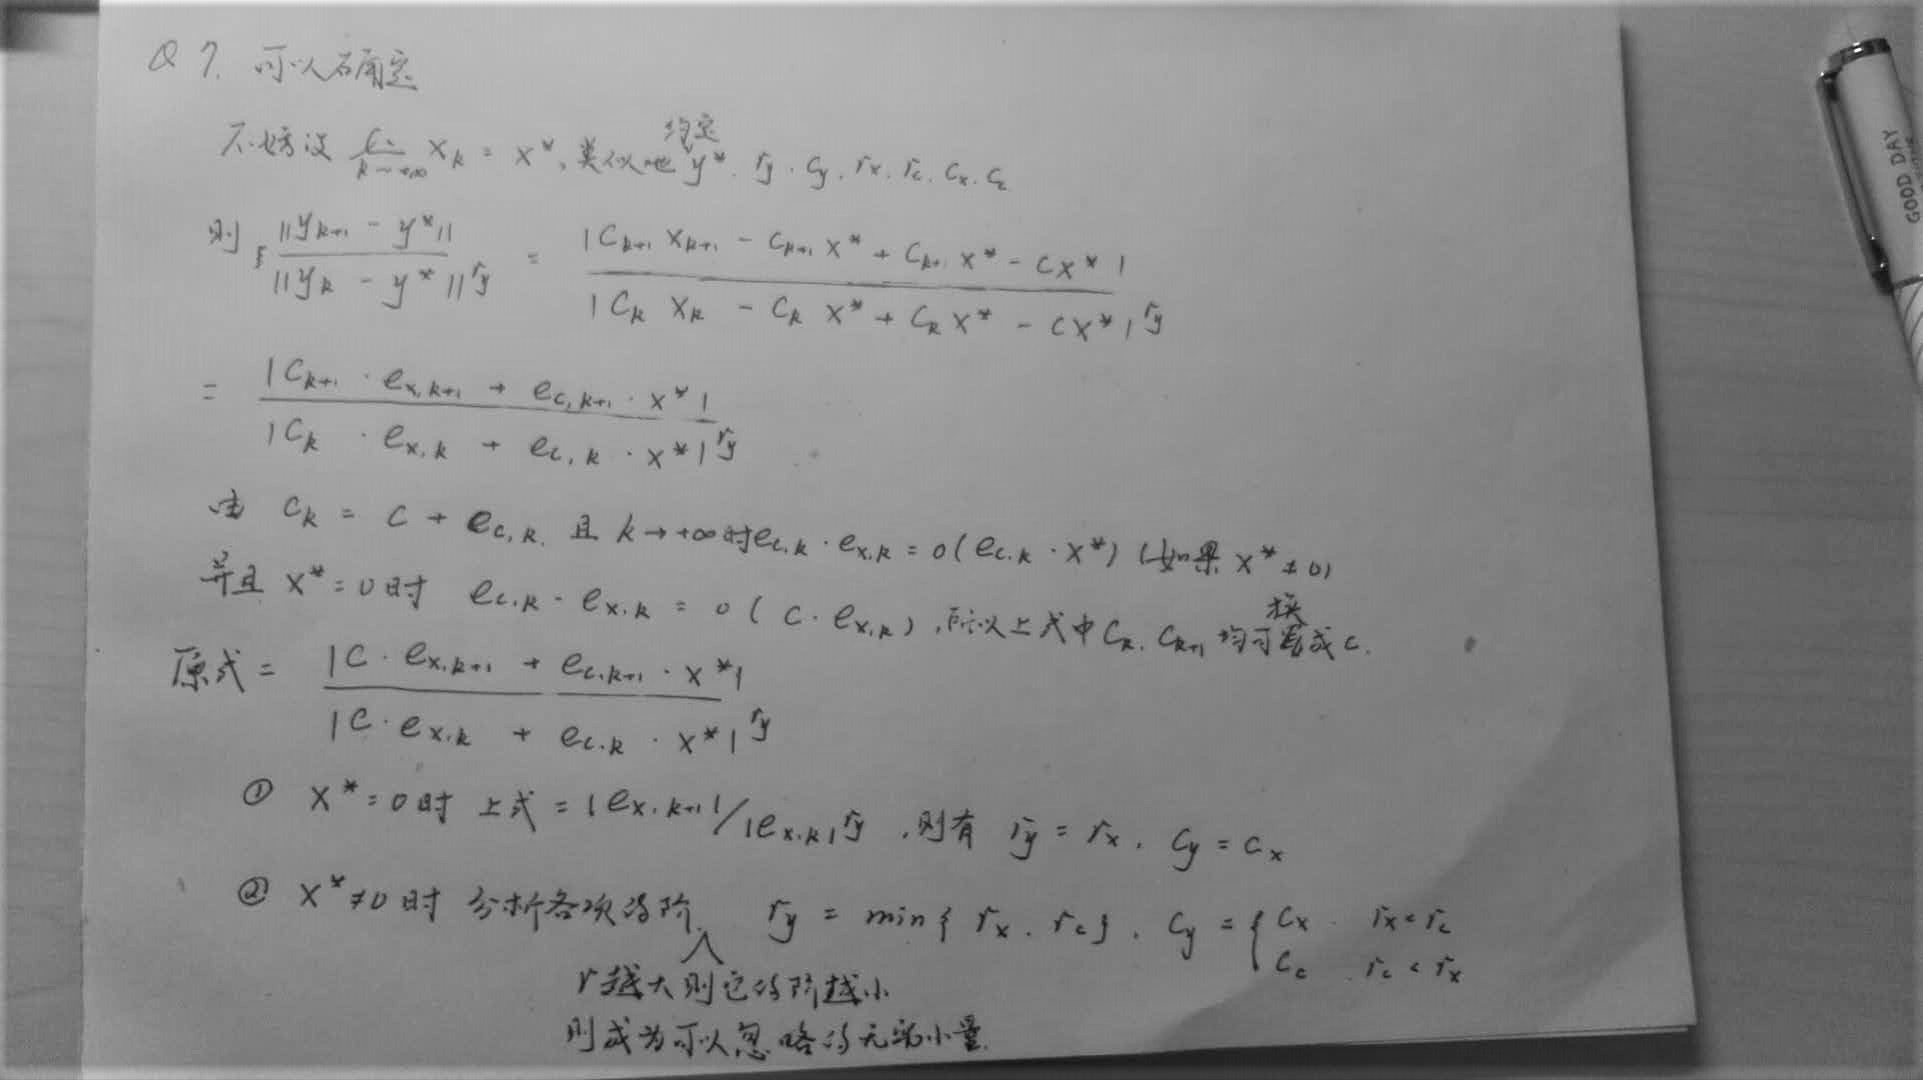
\includegraphics[scale=0.3]{Q7.jpg}
  \caption{Q7}
  \label{fig:label}
\end{figure}

\begin{figure}[ht]
  \centering
  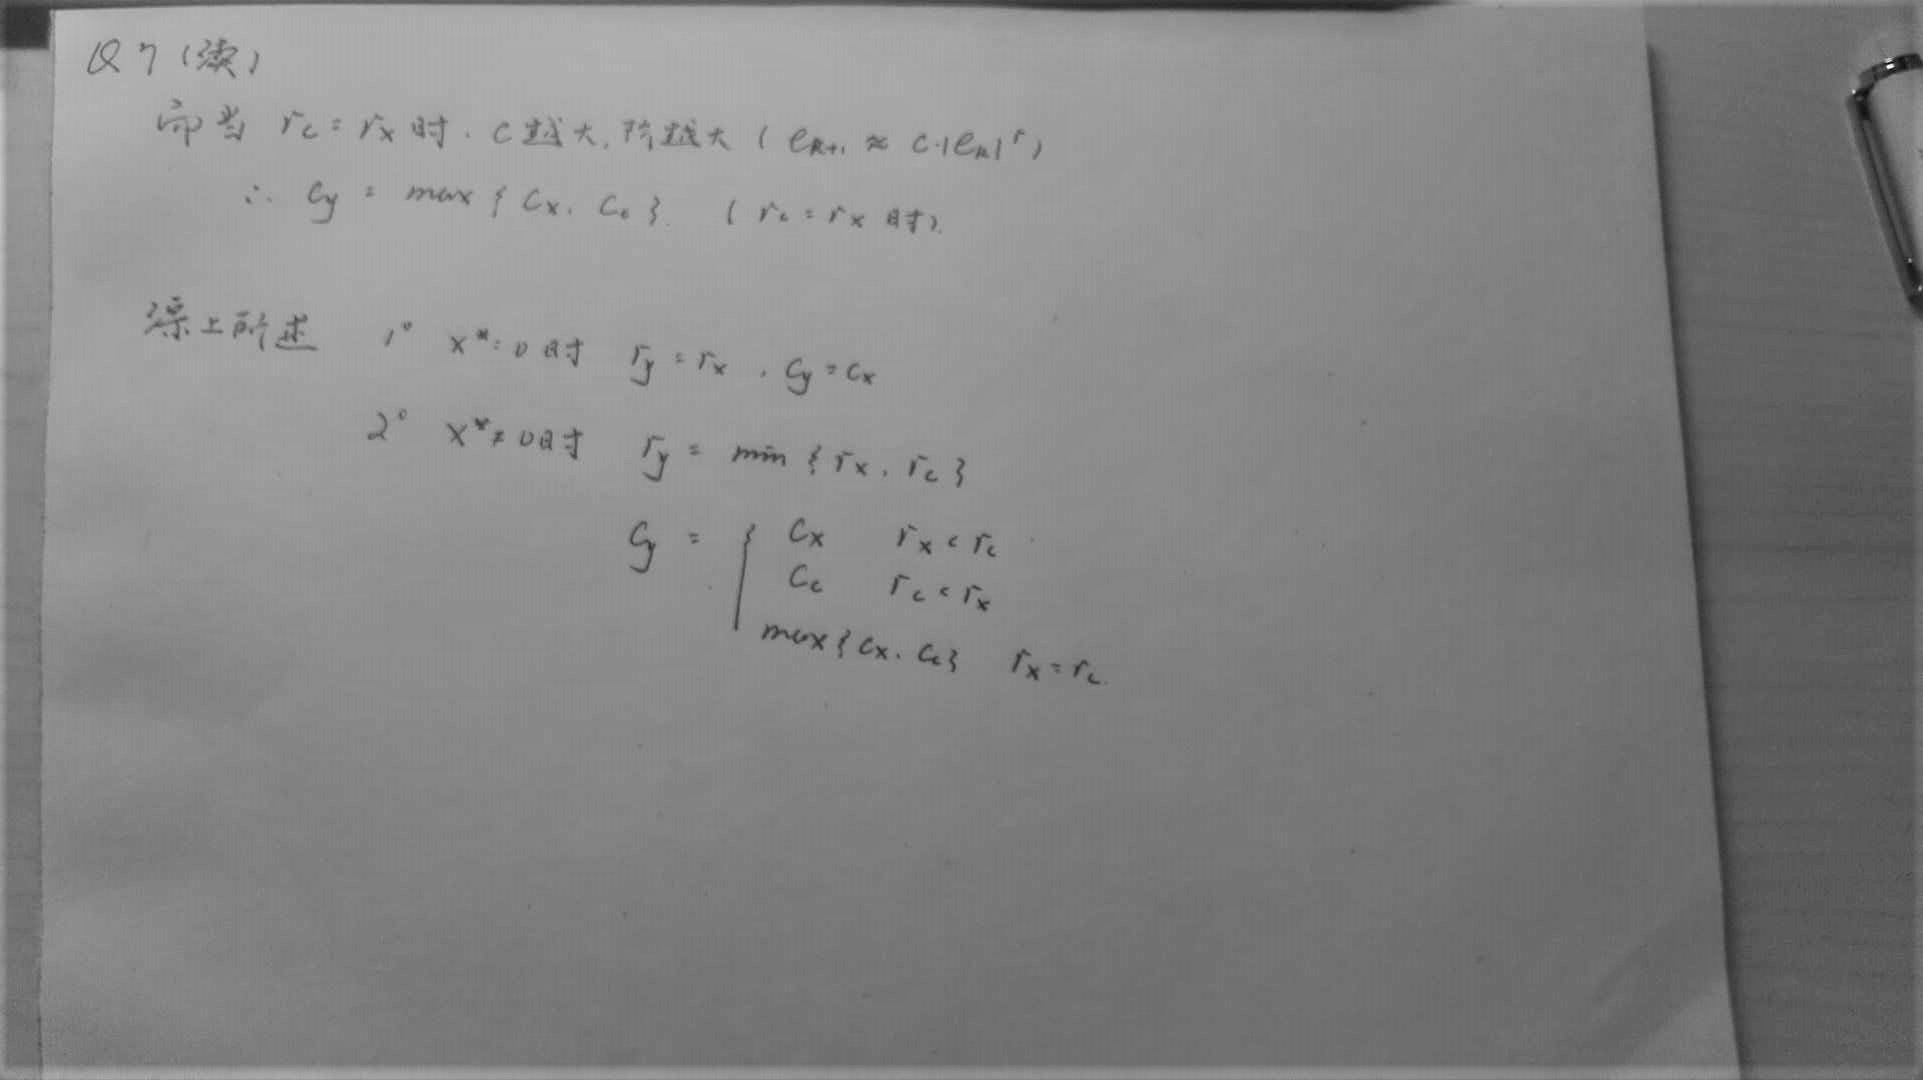
\includegraphics[scale=0.3]{Q7_cont.jpg}
  \caption{Q7cont}
  \label{fig:label}
\end{figure}
\end{document}
